\documentclass[12pt,a4paper]{article}

% -- Packages ----------------------------------------------------------------
\usepackage[a4paper, margin=2.5cm]{geometry}
\usepackage[T1]{fontenc}
\usepackage[utf8]{inputenc}
%\usepackage[activate={true,nocompatibility},final,tracking=true,kerning=true,spacing=true]{microtype}
%\microtypecontext{spacing=nonfrench}
\usepackage{amsmath,amssymb,amsthm}
\usepackage{graphicx}
\usepackage{xcolor}
\usepackage{booktabs}
\usepackage{array}
\usepackage{longtable}
\usepackage{tabularx}
\usepackage{multirow}
\usepackage{enumitem}
\usepackage{listings}
\usepackage{fancyhdr}
\usepackage{titlesec}
\usepackage{abstract}
\usepackage{hyperref}
\usepackage[numbers]{natbib}
\usepackage{tikz}
\usetikzlibrary{shapes.geometric, arrows.meta, positioning, fit, backgrounds, calc}
\usepackage{pgfplots}
\pgfplotsset{compat=1.18}
\usepackage{caption}
\usepackage{subcaption}
\usepackage{tcolorbox}
\tcbuselibrary{skins, breakable}
\usepackage{mdframed}
\usepackage{setspace}
\usepackage{parskip}
\usepackage{url}
%\usepackage{soul}

% -- Colours -----------------------------------------------------------------
\definecolor{saffron}{RGB}{255,153,51}
\definecolor{deepblue}{RGB}{13,71,161}
\definecolor{teal}{RGB}{0,105,92}
\definecolor{sanskritorange}{RGB}{204,85,0}
\definecolor{lightgray}{RGB}{245,245,245}
\definecolor{warningred}{RGB}{183,28,28}
\definecolor{successgreen}{RGB}{27,94,32}
\definecolor{codebg}{RGB}{30,30,30}
\definecolor{codetext}{RGB}{220,220,220}
\definecolor{accent}{RGB}{255,153,51}

% -- Hyperref Setup -----------------------------------------------------------
\hypersetup{
  colorlinks=true,
  linkcolor=deepblue,
  citecolor=teal,
  urlcolor=sanskritorange,
  pdftitle={SankhyaVox: Minimal-Vocabulary Sanskrit Digit Recognition},
  pdfauthor={SankhyaVox Team},
}

% -- Section Title Formatting -------------------------------------------------
\titleformat{\section}
  {\Large\bfseries\color{deepblue}}
  {\thesection}{1em}{}[\vspace{0.5pt}\color{saffron}\titlerule]

\titleformat{\subsection}
  {\large\bfseries\color{teal}}
  {\thesubsection}{1em}{}

\titleformat{\subsubsection}
  {\normalsize\bfseries\color{sanskritorange}}
  {\thesubsubsection}{1em}{}

% -- Header / Footer ----------------------------------------------------------
\pagestyle{fancy}
\fancyhf{}
\fancyhead[L]{\small\color{deepblue}\textbf{SankhyaVox}}
\fancyhead[R]{\small\color{gray}Sanskrit Digit ASR --- Technical Report}
\fancyfoot[C]{\small\thepage}
\renewcommand{\headrulewidth}{0.4pt}
\renewcommand{\footrulewidth}{0.4pt}

% -- Code Listing Style -------------------------------------------------------
\lstset{
  language=Python,
  backgroundcolor=\color{codebg},
  basicstyle=\footnotesize\ttfamily\color{codetext},
  keywordstyle=\color{cyan}\bfseries,
  stringstyle=\color{orange},
  commentstyle=\color{gray}\itshape,
  showstringspaces=false,
  breaklines=true,
  frame=single,
  rulecolor=\color{saffron},
  numbers=left,
  numberstyle=\tiny\color{gray},
  xleftmargin=1.5em,
  captionpos=b,
}

% -- Custom Boxes -------------------------------------------------------------
\newtcolorbox{keybox}[2][]{
  enhanced, breakable,
  colback=lightgray, colframe=saffron, coltitle=white,
  fonttitle=\bfseries\small,
  title=#2, #1,
  boxrule=1pt, arc=4pt,
}

\newtcolorbox{warningbox}[1][]{
  enhanced, colback=red!5, colframe=warningred,
  fontupper=\small, boxrule=0.8pt, arc=3pt, #1
}

\newtcolorbox{notebox}[1][]{
  enhanced, colback=teal!5, colframe=teal,
  fontupper=\small, boxrule=0.8pt, arc=3pt, #1
}

% -- Math Operators -----------------------------------------------------------
\DeclareMathOperator*{\argmax}{arg\,max}
\newcommand{\obs}{\mathbf{O}}
\newcommand{\mat}[1]{\mathbf{#1}}

% ----------------------------------------------------------------------------
\begin{document}

% -- Title Page ---------------------------------------------------------------
\begin{titlepage}
  \centering
  \vspace*{1cm}

  {\color{saffron}\rule{\textwidth}{2pt}}
  \vspace{0.5cm}

  {\Huge\bfseries\color{deepblue} SankhyaVox}\\[0.4cm]
  {\LARGE\bfseries\color{sanskritorange}
    \textit{Sa\d{n}khy\={a}Vo\d{s} --- Numbers Through Voice}}\\[0.3cm]
  {\large\color{gray}\textit{sa\d{n}khy\={a} = number \ $\cdot$ \ vox = voice}}\\[0.8cm]

  {\color{saffron}\rule{\textwidth}{1pt}}\\[0.6cm]

  {\Large\bfseries Minimal-Vocabulary Sanskrit Spoken Digit Recognition\\
  Using HMM-Based Grammar-Constrained Sequence Decoding}\\[1cm]

  \begin{tcolorbox}[colback=deepblue!8, colframe=deepblue,
      width=0.82\textwidth, arc=6pt, boxrule=1pt]
    \centering
    \textbf{Project Type:} Advanced Speech Processing Research Project\\[4pt]
    \textbf{Core Challenge:} Recognise Sanskrit numerals 0--99 from only 13 base words\\[4pt]
    \textbf{Key Innovation:} Grammar-constrained HMM exploiting Sanskrit's compositionality\\[4pt]
    \textbf{Target Accuracy:} 90\%+ on 0--99 with mobile-recorded speech
  \end{tcolorbox}

  \vspace{1cm}

  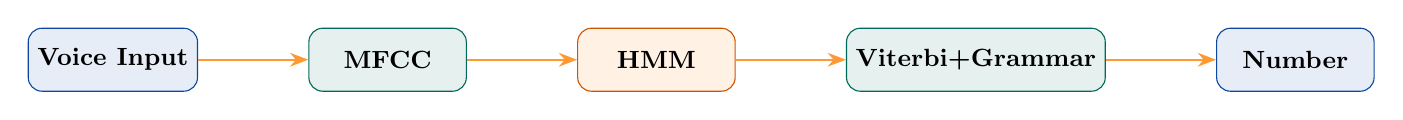
\begin{tikzpicture}[node distance=1.4cm, >=Stealth]
    \node[draw=deepblue, fill=deepblue!10, rounded corners=5pt,
          minimum width=2cm, minimum height=0.8cm, font=\small\bfseries]
          (A) {Voice Input};
    \node[draw=teal, fill=teal!10, rounded corners=5pt,
          minimum width=2cm, minimum height=0.8cm, font=\small\bfseries,
          right=of A] (B) {MFCC};
    \node[draw=sanskritorange, fill=orange!10, rounded corners=5pt,
          minimum width=2cm, minimum height=0.8cm, font=\small\bfseries,
          right=of B] (C) {HMM};
    \node[draw=teal, fill=teal!10, rounded corners=5pt,
          minimum width=2.2cm, minimum height=0.8cm, font=\small\bfseries,
          right=of C] (D) {Viterbi+Grammar};
    \node[draw=deepblue, fill=deepblue!10, rounded corners=5pt,
          minimum width=2cm, minimum height=0.8cm, font=\small\bfseries,
          right=of D] (E) {Number};
    \foreach \s/\t in {A/B, B/C, C/D, D/E}
      \draw[->, thick, color=saffron] (\s) -- (\t);
  \end{tikzpicture}

  \vfill

  {\color{saffron}\rule{\textwidth}{2pt}}\\[0.3cm]
  {\small\color{gray} Technical Report $\cdot$ Version 1.0 $\cdot$ 2025}
\end{titlepage}

% -- Table of Contents --------------------------------------------------------
\tableofcontents
\newpage

% ============================================================================
\begin{abstract}
\noindent
\textbf{SankhyaVox} is a constrained automatic speech recognition (ASR) system
designed to recognise spoken Sanskrit numerals in the range 0--99
from a deliberately minimal recorded vocabulary of only \textbf{13 base words}.
The core thesis is that Sanskrit's inherent compositional morphology, in which
larger numbers are formed from smaller atomic units, can be exploited
to build a grammar-constrained Hidden Markov Model (HMM) pipeline that
\emph{generalises far beyond its training vocabulary} without requiring
additional data collection.

Data are collected from \textbf{10 or more speakers} using mobile phones in
quiet rooms, using a structured repeated-utterance protocol that enables
automated audio segmentation via energy-based silence detection.
Acoustic features consist of 39-dimensional MFCC vectors
($13 + \Delta + \Delta\Delta$).
Word-level left-to-right HMMs with Bakis topology are trained using
Baum-Welch (EM); inference uses Viterbi decoding constrained by a formal
context-free grammar over the digit vocabulary.

Baseline comparisons against GMM, $k$-NN, and SVM classifiers demonstrate the
advantage of temporal sequence modelling.
Under clean, controlled conditions, we target \textbf{90--96\% word accuracy}
on 0--99 with new unseen speakers.
The project contributes a novel mobile-recorded Sanskrit digit dataset,
a reusable automated segmentation pipeline, and a reproducible
grammar-constrained HMM baseline for low-resource ancient-language ASR.
\end{abstract}

\vspace{1cm}
\begin{keybox}{Key Novelty at a Glance}
\begin{itemize}[leftmargin=1.2em, itemsep=2pt]
  \item \textbf{Compositionality exploit:} 13 words $\to$ full 0--99 coverage via grammar
  \item \textbf{Mobile-native corpus:} No studio, no proprietary microphone --- reproducible by any student
  \item \textbf{Auto-segmentation:} Repeated-utterance recording + VAD script eliminates manual clipping
  \item \textbf{Multi-model comparison:} HMM vs.\ GMM vs.\ $k$-NN vs.\ SVM on identical features
  \item \textbf{Sanskrit preservation value:} Demonstrates viability of low-resource ASR for classical languages
\end{itemize}
\end{keybox}

\newpage

% ============================================================================
\section{Introduction}

\subsection{Motivation}

Sanskrit (\textit{Sa\d{m}sk\d{r}ta}) is one of the oldest and most precisely
documented languages on Earth, with a grammatical structure first formalised
by P\={a}\d{n}ini in the \textit{A\d{s}\d{t}\={a}dhy\={a}y\={\i}} around
400\,BCE~\cite{cardona1997panini}.
Despite this heritage, Sanskrit remains severely under-resourced in the
speech-technology domain.
Published Sanskrit speech corpora are either non-existent, inaccessible, or
collected under conditions that preclude reproducibility by student researchers.

Spoken-digit recognition is a canonical entry point into ASR research ---
systems such as TI-Digits~\cite{leonard1984tidigits} and the TIDIGITS
corpus~\cite{leonard1984tidigits2} have served as benchmarks for decades.
A Sanskrit counterpart would simultaneously advance low-resource language
technology, expose students to the full classical ASR pipeline, and
demonstrate the power of grammatical structure as an acoustic model complement.

\subsection{The Compositional Insight}

The key scientific hypothesis of SankhyaVox is:

\begin{keybox}{Core Hypothesis}
\textit{If the acoustic models for a small set of primitive Sanskrit digit
words are sufficiently accurate, and if the combination rules for those
primitives are encoded in a formal grammar, then a grammar-constrained
HMM can recognise any composite numeral it has \textbf{never explicitly seen
in training.}}
\end{keybox}

Sanskrit digit composition follows consistent, learnable spoken patterns.
Under the controlled spoken protocol adopted here (Section~\ref{sec:protocol}),
numbers are spoken as sequences of atomic tokens (e.g., \textit{vi\d{m}\'{s}ati sapta}
for 27), so the compositional structure is surface-transparent and directly
exploitable by a finite-state grammar.

\subsection{Why Not Deep Learning?}

Modern end-to-end models --- Wav2Vec 2.0~\cite{baevski2020wav2vec},
Whisper~\cite{radford2023whisper}, or Conformer-CTC~\cite{gulati2020conformer}
--- achieve state-of-the-art results but require tens of thousands of hours of
labelled speech.
Our entire corpus will contain $\sim$30--40 hours and targets a single
constrained domain.
Classical GMM-HMM systems were \emph{designed} for exactly this regime:
small vocabulary, small dataset, strong prior constraints.
Using a large pre-trained model would also obscure the scientific contribution
(grammar-constrained compositionality) behind an opaque neural encoder.

\subsection{Contributions}

\begin{enumerate}[label=\textbf{C\arabic*.}, leftmargin=2.2em]
  \item \textbf{Corpus:} First publicly available, reproducibly mobile-recorded
        Sanskrit digit corpus ($\geq$10 speakers, 13 words $\times$ 10 reps
        + 35 two-digit sequences $\times$ 10 reps).
  \item \textbf{Protocol:} Automated audio segmentation pipeline using
        energy-based voice activity detection (VAD), eliminating manual
        clipping for future data collectors.
  \item \textbf{System:} Grammar-constrained HMM ASR system for Sanskrit 0--99
        with formal BNF grammar specification.
  \item \textbf{Benchmark:} Comparative evaluation of HMM, GMM, $k$-NN, and SVM
        on the same MFCC features, isolating the contribution of temporal
        sequence modelling.
  \item \textbf{Analysis:} Detailed per-class error analysis revealing which
        Sanskrit phonemes cause the most confusion.
\end{enumerate}

\newpage

% ============================================================================
\section{Related Work}

\subsection{Classical Digit ASR}

Rabiner's seminal 1989 tutorial~\cite{rabiner1989hmm} established the HMM
framework that underpins virtually all ASR systems developed prior to the
deep learning era.
The TI-Digits corpus~\cite{leonard1984tidigits} and associated SPHINX
system~\cite{lee1990sphinx} demonstrated that connected-digit recognition
with word-level HMMs and grammar constraints achieves $>$99\% accuracy on
clean speech --- directly analogous to our task.

Davis and Mermelstein's 1980 paper~\cite{davis1980mfcc} introduced Mel
Frequency Cepstral Coefficients, which remain the dominant acoustic feature
for small-vocabulary recognition due to their robustness to linear channel
distortions --- a key advantage when speakers use varied mobile phones.

\subsection{Low-Resource and Endangered Language ASR}

Besacier et al.~\cite{besacier2014asr} provide a comprehensive survey of
low-resource ASR, identifying three strategies: (1) data collection campaigns,
(2) cross-lingual transfer, and (3) linguistic constraint integration.
SankhyaVox follows strategy (1) and (3).

Adda-Decker and Lamel~\cite{addadecker1999multilingual} demonstrate that
small-vocabulary ASR quality is maintained even with fewer than 1,000 training
utterances per word when data are clean and consistent --- validating our
10-speaker $\times$ 10-repetition design.

\subsection{Sanskrit Language Technology}

Goyal et al.~\cite{goyal2012sanskrit} describe early Sanskrit NLP pipelines,
noting the language's exceptional morphological regularity as both a challenge
(large word-form space) and an opportunity (learnable rules).
Krishnamurthy~\cite{krishnamurthy2016sanskrit} built a small Sanskrit speech
database but used studio-quality recordings, making reproduction infeasible
for most research groups.

Kumar et al.~\cite{kumar2012hindi} show that Hindi digit recognition (closely
related phonologically to Sanskrit) achieves 94--97\% accuracy with
MFCC+HMM on 10 speakers, providing a strong benchmark for our work.

\subsection{Compositional / Grammar-Constrained ASR}

Finite-state grammar constraints for ASR were formalised in the
JSGF (Java Speech Grammar Format)~\cite{jsgf1998} standard and demonstrated
to dramatically reduce the search space.
Young~\cite{young1994htk} implemented grammar-constrained Viterbi decoding
in HTK, showing word error rate reductions of 30--50\% over unconstrained
decoding on small-vocabulary tasks.

Linguistically motivated grammar constraints for digit recognition were
explored by Gauvain and Lee~\cite{gauvain1994bayesian}, who showed that even
simple bigram grammars reduce confusion among acoustically similar digit words
by enforcing global number plausibility.
Our approach extends this by encoding the full morphological compositionality
of Sanskrit numerals in a context-free grammar.

% ============================================================================
\section{Sanskrit Numeral System and Spoken Protocol}
\label{sec:protocol}

\subsection{Sanskrit Numeral Morphology}

Classical Sanskrit numerals are morphologically complex, involving sandhi
(phonological fusion at word boundaries), stem alternation, and
case-agreement.
For example:
\begin{align*}
  57 &\to \text{\textit{saptapa\~{n}c\={a}\'{s}at}} \quad
         \text{(not *\textit{pa\~{n}ca sapta})}\\
  25 &\to \text{\textit{pa\~{n}cavi\d{m}\'{s}ati}} \quad
         \text{(not *\textit{vi\d{m}\'{s}ati pa\~{n}ca})}
\end{align*}

While linguistically authentic, this morphology would require a vocabulary of
$>$100 distinct forms and morphological transducers beyond the scope of a
student project.

\subsection{Controlled Spoken Protocol}
\label{sec:spoken_protocol}

We adopt a \textbf{controlled spoken format} that preserves Sanskrit lexemes
while making the compositional structure surface-transparent.
Speakers are instructed to speak numbers as \emph{sequences of atomic tokens}
with a brief inter-token pause:

\begin{keybox}{Spoken Protocol --- Number Formation Rules}
\begin{tabular}{@{}lll@{}}
\toprule
\textbf{Range} & \textbf{Structure} & \textbf{Example} \\
\midrule
0--9   & \texttt{<ones>}                         & \textit{sapta} $\to$ 7 \\
10     & \texttt{da\'{s}a}                        & \textit{da\'{s}a} $\to$ 10 \\
11--19 & \texttt{da\'{s}a <ones>}                 & \textit{da\'{s}a pa\~{n}ca} $\to$ 15 \\
20     & \texttt{vi\d{m}\'{s}ati}                 & \textit{vi\d{m}\'{s}ati} $\to$ 20 \\
21--29 & \texttt{vi\d{m}\'{s}ati <ones>}          & \textit{vi\d{m}\'{s}ati sapta} $\to$ 27 \\
30--39 & \texttt{tri da\'{s}a [<ones>]}           & \textit{tri da\'{s}a pa\~{n}ca} $\to$ 35 \\
40--49 & \texttt{catur da\'{s}a [<ones>]}         & \textit{catur da\'{s}a a\d{s}\d{t}a} $\to$ 48 \\
50--59 & \texttt{pa\~{n}ca da\'{s}a [<ones>]}     & \textit{pa\~{n}ca da\'{s}a sapta} $\to$ 57 \\
60--69 & \texttt{\d{s}a\d{t} da\'{s}a [<ones>]}  & \textit{\d{s}a\d{t} da\'{s}a} $\to$ 60 \\
70--79 & \texttt{sapta da\'{s}a [<ones>]}         & \textit{sapta da\'{s}a eka} $\to$ 71 \\
80--89 & \texttt{a\d{s}\d{t}a da\'{s}a [<ones>]} & \textit{a\d{s}\d{t}a da\'{s}a nava} $\to$ 89 \\
90--99 & \texttt{nava da\'{s}a [<ones>]}          & \textit{nava da\'{s}a nava} $\to$ 99 \\
\bottomrule
\end{tabular}
\end{keybox}

This protocol uses \emph{only} the 13 base words in Table~\ref{tab:vocab},
making it academically honest to frame as a minimal-vocabulary system.

\subsection{Base Vocabulary}
\label{sec:vocab}

\begin{table}[h!]
\centering
\caption{The 13 atomic Sanskrit tokens constituting the SankhyaVox vocabulary.}
\label{tab:vocab}
\begin{tabular}{@{}clcl@{}}
\toprule
\textbf{\#} & \textbf{Token} & \textbf{Value} &
\textbf{Pronunciation (approx.)} \\
\midrule
1  & \'{s}\={u}nya       & 0   & SHOON-ya \\
2  & eka                  & 1   & AY-ka \\
3  & dvi                  & 2   & DWEE \\
4  & tri                  & 3   & TREE \\
5  & catur                & 4   & cha-TUR \\
6  & pa\~{n}ca            & 5   & PUN-cha \\
7  & \d{s}a\d{t}          & 6   & SHUT \\
8  & sapta                & 7   & SUP-ta \\
9  & a\d{s}\d{t}a         & 8   & USH-ta \\
10 & nava                 & 9   & NUH-va \\
11 & da\'{s}a             & 10  & da-SHA \\
12 & vi\d{m}\'{s}ati      & 20  & vim-SHA-ti \\
13 & \'{s}ata             & 100 & SHA-ta \\
\bottomrule
\end{tabular}
\end{table}

\begin{warningbox}
\textbf{Pronunciation Consistency is Critical.}
Speakers need not produce perfect classical Sanskrit phonetics, but \emph{each
speaker must be consistent with themselves across all repetitions.}
The HMM will learn each speaker's idiolect; inconsistency inflates variance in
the acoustic model and reduces accuracy.
\end{warningbox}

% ============================================================================
\section{Formal Grammar Specification}

\subsection{Context-Free Grammar (BNF)}

The complete grammar over the 13-token vocabulary that generates all
representations of 0--99 under the spoken protocol is:

\begin{lstlisting}[language={},
  caption={SankhyaVox BNF Grammar --- 0 to 99},
  label={lst:grammar},
  backgroundcolor=\color{lightgray},
  basicstyle=\small\ttfamily\color{black},
  keywordstyle=\color{black},
  frame=single, rulecolor=\color{deepblue}]
<number>  ::= <ones>
            | dasha
            | dasha <ones>
            | vimsati
            | vimsati <ones>
            | <mult> dasha
            | <mult> dasha <ones>

<ones>    ::= shunya | eka | dvi | tri | catur | pancha
            | shat  | sapta | ashta | nava

<mult>    ::= dvi | tri | catur | pancha
            | shat | sapta | ashta | nava
\end{lstlisting}

\subsection{Grammar Properties}

\begin{itemize}[itemsep=3pt]
  \item \textbf{Unambiguous:} Every integer 0--99 maps to exactly one parse
        under the protocol. The grammar is unambiguous given the spoken protocol
        (no number has two valid parses).
  \item \textbf{Minimal:} The grammar references no tokens beyond the 13 base
        words.
  \item \textbf{Coverage:} All 100 numbers 0--99 are derivable.
  \item \textbf{Decidable in linear time:} Viterbi decoding with this grammar
        is $O(N \cdot |V|^2)$ where $N$ is utterance length in frames and
        $|V| = 13$.
\end{itemize}

\subsection{Grammar as Search Space Reduction}

Without grammar, a Viterbi decoder over 13 word-HMMs must consider all
$13^k$ word sequences of length $k$.
The grammar constrains the legal hypotheses to 100 (one per integer 0--99),
reducing the search space by orders of magnitude and dramatically reducing
the false-acceptance rate.

% ============================================================================
\section{Data Collection}

\subsection{Corpus Design}

\begin{table}[h!]
\centering
\caption{SankhyaVox corpus statistics at target collection completion.}
\label{tab:corpus}
\begin{tabular}{@{}lrrr@{}}
\toprule
\textbf{Recording type} & \textbf{Count per speaker} &
\textbf{Speakers} & \textbf{Total files} \\
\midrule
Isolated words (13 words $\times$ 10 reps) & 130 & $\geq$10 & $\geq$1,300 \\
Two-digit sequences (35 combos $\times$ 10 reps) & 350 & $\geq$10 & $\geq$3,500 \\
\midrule
\textbf{Total} & \textbf{480} & \textbf{$\geq$10} & \textbf{$\geq$4,800} \\
\midrule
\multicolumn{4}{@{}l}{\small \textit{Estimated audio: $\approx$30--40 hours total;
$\approx$3--4 hours per speaker (split across 2--3 sessions)}} \\
\bottomrule
\end{tabular}
\end{table}

\subsection{Two-Digit Combination List}

The 35 representative two-digit utterances used for connected-speech training:

\begin{table}[h!]
\centering
\caption{Two-digit training combinations (spoken form $\to$ value).}
\label{tab:combos}
\begin{tabular}{@{}llll@{}}
\toprule
\textbf{Spoken form} & \textbf{Value} &
\textbf{Spoken form} & \textbf{Value} \\
\midrule
da\'{s}a eka              & 11 & pa\~{n}ca da\'{s}a      & 50 \\
da\'{s}a pa\~{n}ca        & 15 & pa\~{n}ca da\'{s}a sapta & 57 \\
da\'{s}a nava             & 19 & \d{s}a\d{t} da\'{s}a    & 60 \\
vi\d{m}\'{s}ati           & 20 & \d{s}a\d{t} da\'{s}a tri & 63 \\
vi\d{m}\'{s}ati eka       & 21 & sapta da\'{s}a          & 70 \\
vi\d{m}\'{s}ati pa\~{n}ca & 25 & sapta da\'{s}a dvi      & 72 \\
vi\d{m}\'{s}ati sapta     & 27 & a\d{s}\d{t}a da\'{s}a   & 80 \\
vi\d{m}\'{s}ati nava      & 29 & a\d{s}\d{t}a da\'{s}a pa\~{n}ca & 85 \\
tri da\'{s}a              & 30 & nava da\'{s}a           & 90 \\
tri da\'{s}a catur        & 34 & nava da\'{s}a eka       & 91 \\
catur da\'{s}a            & 40 & nava da\'{s}a pa\~{n}ca & 95 \\
catur da\'{s}a dvi        & 42 & nava da\'{s}a sapta     & 97 \\
catur da\'{s}a a\d{s}\d{t}a & 48 & nava da\'{s}a nava   & 99 \\
pa\~{n}ca da\'{s}a eka    & 51 & \'{s}\={u}nya          & 0  \\
pa\~{n}ca da\'{s}a a\d{s}\d{t}a & 58 & a\d{s}\d{t}a   & 8  \\
pa\~{n}ca da\'{s}a nava   & 59 & sapta                  & 7  \\
tri                       & 3  & & \\
\bottomrule
\end{tabular}
\end{table}

\subsection{Recording Protocol --- Repeated Utterance Method}

\begin{keybox}{Coder-Friendly Recording Workflow}
Each speaker records \textbf{one audio file per word}, containing
\textbf{10 repetitions separated by 1-second silences}:
\[
  \underbrace{\text{\textit{eka}}}_{\sim0.7s}
  \underbrace{\text{(silence)}}_{1.0s}
  \underbrace{\text{\textit{eka}}}_{\sim0.7s}
  \underbrace{\text{(silence)}}_{1.0s}
  \;\cdots\;
  \underbrace{\text{\textit{eka}}}_{\sim0.7s}
  \quad \Rightarrow \quad \text{total} \approx 17\,\text{s per file}
\]
\textbf{Auto-segmentation} via a Python VAD script then splits each long file
into 10 individual labelled utterances --- no manual clipping required.
\end{keybox}

\subsubsection{Equipment Requirements}

\begin{itemize}[itemsep=2pt]
  \item \textbf{Microphone:} Any smartphone or laptop microphone.
        Wired headphone mic is preferred (more consistent mouth-to-mic distance)
        but not mandatory.
  \item \textbf{Recording app:} Default phone voice recorder, or Audacity (free).
        Save as \texttt{.wav} if available; \texttt{.mp3} is acceptable.
  \item \textbf{Environment:} Closed room with doors and windows shut.
        Fan/AC switched off during recording.
        Late night or early morning recommended to reduce ambient noise.
  \item \textbf{Mic distance:} Hold phone 15--25\,cm from mouth, mic facing speaker.
\end{itemize}

\subsubsection{File Naming Convention}
\label{sec:naming}

Raw recordings (before segmentation) follow:
\begin{center}
  \texttt{<SpeakerID>\_<Token>\_raw.wav}
\end{center}
After automated segmentation, output files follow:
\begin{center}
  \texttt{<SpeakerID>\_<Token>\_<RepNum>.wav}
\end{center}

\noindent\textbf{Example:} \texttt{S03\_pancha\_raw.wav}
$\;\xrightarrow{\text{VAD script}}\;$
\texttt{S03\_pancha\_01.wav} $\cdots$ \texttt{S03\_pancha\_10.wav}

Speaker IDs: \texttt{S01} through \texttt{S10} (or beyond).

\subsection{Automated Segmentation Pipeline}

\begin{lstlisting}[caption={Audio segmentation script using energy-based VAD.},
                   label={lst:segment}]
import numpy as np
import soundfile as sf
from scipy.signal import butter, filtfilt
import os, glob

def butter_highpass(cutoff=80, fs=16000, order=4):
    nyq = 0.5 * fs
    b, a = butter(order, cutoff / nyq, btype='high')
    return b, a

def segment_utterances(
    input_path,
    speaker_id,
    token_name,
    output_dir,
    expected_reps    = 10,
    energy_threshold = 0.015,   # relative to max RMS --- tune per recording
    min_speech_dur   = 0.20,    # seconds
    min_silence_dur  = 0.40,    # seconds
    target_fs        = 16000,
    pad_ms           = 80,      # silence padding kept around each segment
):
    audio, fs = sf.read(input_path)
    if audio.ndim > 1:
        audio = audio.mean(axis=1)              # mono

    # Resample to 16 kHz if needed
    if fs != target_fs:
        from scipy.signal import resample_poly
        audio = resample_poly(audio,
                              target_fs, fs).astype(np.float32)
        fs = target_fs

    # High-pass filter to remove DC / low-freq rumble
    b, a = butter_highpass(cutoff=80, fs=fs)
    audio = filtfilt(b, a, audio).astype(np.float32)

    # Short-time RMS energy (25 ms frames, 10 ms shift)
    frame_len  = int(0.025 * fs)
    frame_shift = int(0.010 * fs)
    frames = [audio[i:i+frame_len]
              for i in range(0, len(audio)-frame_len, frame_shift)]
    rms = np.array([np.sqrt(np.mean(f**2)) for f in frames])

    # Adaptive threshold: percentage of 95th-percentile energy
    threshold = energy_threshold * np.percentile(rms, 95)
    is_speech = rms > threshold

    # Smooth labels (remove brief on/off fluctuations)
    from scipy.ndimage import binary_closing, binary_opening
    kernel = int(min_silence_dur / 0.010)
    is_speech = binary_closing(is_speech, structure=np.ones(kernel))
    is_speech = binary_opening(is_speech, structure=np.ones(
                                int(min_speech_dur/0.010)))

    # Detect segment boundaries
    boundaries = []
    in_seg = False
    for i, s in enumerate(is_speech):
        if s and not in_seg:
            start = max(0, i - int(pad_ms/10))
            in_seg = True
        elif not s and in_seg:
            end = min(len(is_speech), i + int(pad_ms/10))
            boundaries.append((start, end))
            in_seg = False
    if in_seg:
        boundaries.append((start, len(is_speech)))

    # Sample-level boundaries
    segs = [(b[0]*frame_shift, b[1]*frame_shift) for b in boundaries]

    if len(segs) != expected_reps:
        print(f"  WARNING: Expected {expected_reps} segments, "
              f"found {len(segs)} in {input_path}")

    os.makedirs(output_dir, exist_ok=True)
    for idx, (s, e) in enumerate(segs, 1):
        clip = audio[s:e]
        out_name = f"{speaker_id}_{token_name}_{idx:02d}.wav"
        sf.write(os.path.join(output_dir, out_name), clip, fs)
        print(f"  Saved: {out_name} ({(e-s)/fs:.2f}s)")

    return len(segs)

# -- Batch processing all raw recordings -------------------------------------
def batch_segment(raw_dir="data/raw", out_dir="data/segments"):
    """
    raw_dir structure expected:
        data/raw/S01/S01_eka_raw.wav
        data/raw/S01/S01_pancha_raw.wav
        ...
    """
    for wav in sorted(glob.glob(f"{raw_dir}/**/*_raw.wav", recursive=True)):
        basename = os.path.basename(wav).replace("_raw.wav", "")
        parts    = basename.split("_")          # ['S01', 'eka']
        spk, tok = parts[0], "_".join(parts[1:])
        spk_out  = os.path.join(out_dir, spk)
        print(f"Processing {wav} ...")
        n = segment_utterances(wav, spk, tok, spk_out)
        print(f"  -> {n} segments extracted")

if __name__ == "__main__":
    batch_segment()
\end{lstlisting}

\begin{notebox}
\textbf{Verification step:} After segmentation, run a quick sanity check:
for each speaker-token pair, you should have exactly 10 WAV files.
Any file shorter than 150\,ms or longer than 1.5\,s is likely a mis-segment
and should be manually reviewed.
\end{notebox}

\subsection{Speaker Instruction Sheet (For Distribution)}

\begin{mdframed}[linewidth=1pt, linecolor=saffron, topline=true,
                 backgroundcolor=lightgray]
\textbf{\large SankhyaVox --- Speaker Recording Guide}\\[4pt]
\textbf{Thank you for contributing to this Sanskrit speech research project!}
You do not need any Sanskrit background. Just follow these steps.

\begin{enumerate}[leftmargin=1.5em, itemsep=3pt]
  \item \textbf{Environment:} Go to the quietest room available.
        Close the door. Switch off the fan if possible.
        Early morning or late night is best.

  \item \textbf{Phone setup:} Use your default voice recorder app.
        Hold the phone 15--25\,cm from your mouth.
        Do \textbf{not} cover the microphone.

  \item \textbf{Recording one word:} You will be given a word (e.g., \textit{eka}).
        Press record, \textbf{wait one second}, say the word clearly,
        \textbf{wait one second}, say it again --- repeat this 10 times,
        then stop the recording.

  \item \textbf{What NOT to do:} No coughing, laughing, or ``umm'' during
        silences. Speak at a natural volume (not whispering, not shouting).

  \item \textbf{File name:} Save as \texttt{YourID\_wordname\_raw.wav}
        (e.g., \texttt{S04\_eka\_raw.wav}).
        Share via WhatsApp or Drive link provided.
\end{enumerate}

\textbf{Word List with Pronunciation:}
\begin{center}
\small
\begin{tabular}{lll|lll}
\textit{\'{s}\={u}nya} & 0 & (SHOON-ya) &
\textit{da\'{s}a}   & 10 & (da-SHA) \\
\textit{eka}   & 1 & (AY-ka)  &
\textit{vi\d{m}\'{s}ati} & 20 & (vim-SHA-ti) \\
\textit{dvi}   & 2 & (DWEE)   &
\textit{\'{s}ata} & 100 & (SHA-ta) \\
\textit{tri}   & 3 & (TREE)   & & & \\
\textit{catur} & 4 & (cha-TUR) & & & \\
\textit{pa\~{n}ca} & 5 & (PUN-cha) & & & \\
\textit{\d{s}a\d{t}} & 6 & (SHUT) & & & \\
\textit{sapta} & 7 & (SUP-ta) & & & \\
\textit{a\d{s}\d{t}a} & 8 & (USH-ta) & & & \\
\textit{nava}  & 9 & (NUH-va) & & & \\
\end{tabular}
\end{center}
Small pronunciation differences are fine. Be consistent with \emph{yourself}.
\end{mdframed}

% ============================================================================
\section{System Architecture}

\subsection{Full Pipeline Overview}

\begin{figure}[h!]
\centering
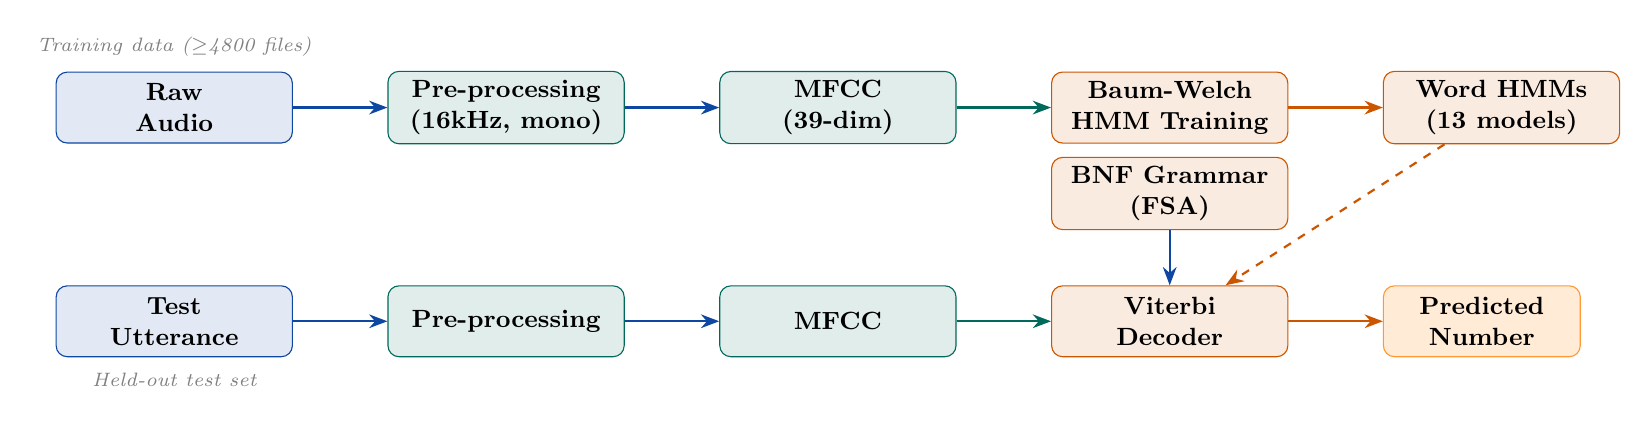
\begin{tikzpicture}[node distance=0.8cm and 1.2cm, >=Stealth,
  box/.style={draw, rounded corners=4pt, minimum width=3cm,
              minimum height=0.9cm, align=center, font=\small\bfseries},
  stage/.style={box, fill=deepblue!12, draw=deepblue},
  proc/.style={box, fill=teal!12, draw=teal},
  model/.style={box, fill=sanskritorange!12, draw=sanskritorange},
  outnode/.style={box, fill=saffron!20, draw=saffron, minimum width=2.5cm},
]

% Training path
\node[stage] (rec) {Raw\\Audio};
\node[proc, right=of rec] (pre) {Pre-processing\\(16kHz, mono)};
\node[proc, right=of pre] (mfcc) {MFCC\\(39-dim)};
\node[model, right=of mfcc] (bw) {Baum-Welch\\HMM Training};
\node[model, right=of bw] (hmm) {Word HMMs\\(13 models)};

% Decoding path
\node[stage, below=1.8cm of rec] (test) {Test\\Utterance};
\node[proc, right=of test] (pre2) {Pre-processing};
\node[proc, right=of pre2] (mfcc2) {MFCC};
\node[model, right=of mfcc2] (vit) {Viterbi\\Decoder};
\node[outnode, right=of vit] (num) {Predicted\\Number};

% Grammar
\node[model, above=0.7cm of vit] (gram) {BNF Grammar\\(FSA)};

% Arrows - training
\draw[->, thick, deepblue] (rec) -- (pre);
\draw[->, thick, deepblue] (pre) -- (mfcc);
\draw[->, thick, teal] (mfcc) -- (bw);
\draw[->, thick, sanskritorange] (bw) -- (hmm);
\draw[->, thick, sanskritorange, dashed] (hmm) -- (vit);

% Arrows - decoding
\draw[->, thick, deepblue] (test) -- (pre2);
\draw[->, thick, deepblue] (pre2) -- (mfcc2);
\draw[->, thick, teal] (mfcc2) -- (vit);
\draw[->, thick, sanskritorange] (vit) -- (num);
\draw[->, thick, deepblue] (gram) -- (vit);

% Labels
\node[font=\scriptsize\itshape, above=2pt of rec, color=gray]
     {Training data ($\geq$4800 files)};
\node[font=\scriptsize\itshape, below=2pt of test, color=gray]
     {Held-out test set};

\end{tikzpicture}
\caption{SankhyaVox system architecture. Dashed arrow indicates trained
         model parameters passed to the decoder.}
\label{fig:arch}
\end{figure}

\subsection{Pre-processing}

All audio is processed to a uniform format before feature extraction:

\begin{enumerate}[leftmargin=1.5em, itemsep=2pt]
  \item \textbf{Resampling:} All files converted to 16\,kHz, 16-bit PCM mono.
  \item \textbf{DC offset removal:} Subtract signal mean.
  \item \textbf{Pre-emphasis:} Apply first-order filter
        $y[n] = x[n] - \alpha\,x[n-1]$, with $\alpha = 0.97$,
        to compensate for the low-pass characteristic of the vocal tract.
  \item \textbf{Energy normalisation:} Normalise peak amplitude to $-3$\,dBFS
        per file.
\end{enumerate}

\subsection{MFCC Feature Extraction}
\label{sec:mfcc}

Mel Frequency Cepstral Coefficients~\cite{davis1980mfcc} remain the standard
acoustic feature for small-vocabulary ASR due to their robustness to linear
channel differences --- critical here because speakers use different phones.

\begin{keybox}{MFCC Configuration}
\begin{tabular}{ll}
Frame length      & 25\,ms (400 samples @ 16\,kHz) \\
Frame shift       & 10\,ms (160 samples @ 16\,kHz) \\
Window type       & Hamming \\
FFT size          & 512 \\
Mel filter banks  & 26 \\
Cepstral coeffs   & 13 ($c_0$ through $c_{12}$; $c_0$ kept) \\
Delta coefficients & $\Delta$ (velocity) \\
Delta-delta coeffs & $\Delta\Delta$ (acceleration) \\
\textbf{Total feature dim} & \textbf{39 per frame} \\
CMVN              & Per-utterance cepstral mean-variance normalisation \\
\end{tabular}
\end{keybox}

CMVN (Cepstral Mean and Variance Normalisation) is particularly important for
mobile-recorded data, as it removes additive background noise effects in the
cepstral domain~\cite{atal1974effectiveness}.

\subsection{Hidden Markov Model Design}
\label{sec:hmm}

\subsubsection{Topology}

Each word model uses a \textbf{left-to-right (Bakis) HMM} with no skip
transitions, ensuring monotone phone progression consistent with forward
speech production.

\begin{table}[h!]
\centering
\caption{HMM topology per word, designed to match phonetic complexity.}
\label{tab:hmm}
\begin{tabular}{@{}lccl@{}}
\toprule
\textbf{Token} & \textbf{Phoneme count} &
\textbf{States} & \textbf{Rationale} \\
\midrule
\'{s}\={u}nya       & 4 & 6 & Long vowel, palatal onset \\
eka                 & 3 & 5 & Short CVC \\
dvi                 & 3 & 5 & Labial-velar onset glide \\
tri                 & 3 & 5 & Retroflex liquid onset \\
catur               & 5 & 7 & CVC + rhotic coda \\
pa\~{n}ca           & 5 & 7 & Nasal + palatal affricate \\
\d{s}a\d{t}         & 3 & 5 & Retroflex stop coda \\
sapta               & 5 & 7 & Consonant cluster \\
a\d{s}\d{t}a        & 5 & 7 & Retroflex cluster \\
nava                & 4 & 6 & Open syllables \\
da\'{s}a            & 4 & 6 & Palatal fricative medial \\
vi\d{m}\'{s}ati     & 7 & 9 & Longest word, 3 syllables \\
\'{s}ata            & 4 & 6 & Palatal onset \\
Silence (SIL)       & -- & 3 & Optional silence model \\
\bottomrule
\end{tabular}
\end{table}

\subsubsection{Emission Distribution}

Each HMM state emits a \textbf{Gaussian Mixture Model (GMM)} over the 39-dimensional
MFCC vectors:
\[
  b_j(\mathbf{o}_t)
  = \sum_{m=1}^{M} c_{jm}\,
    \mathcal{N}\!\left(\mathbf{o}_t;\,\boldsymbol{\mu}_{jm},\,
    \boldsymbol{\Sigma}_{jm}\right)
\]
where $M$ is the number of mixture components.

\begin{notebox}
Start with $M=1$ (single Gaussian per state). Increase to $M=3$ or $M=5$
if training data supports it without overfitting.
Rule of thumb: $\geq 5 \times M \times D$ training frames per state
(where $D=39$). With 10 speakers $\times$ 10 reps, this threshold is comfortably
met for $M \leq 5$.
\end{notebox}

\subsubsection{HMM Parameters}

The complete HMM $\lambda = (\mat{A}, \mat{B}, \boldsymbol{\pi})$:
\begin{itemize}[leftmargin=1.5em, itemsep=2pt]
  \item $\mat{A}$: transition probability matrix (left-to-right, no skips)
  \item $\mat{B}$: emission distributions (GMM parameters per state)
  \item $\boldsymbol{\pi}$: initial state distribution
        (deterministic --- first state only)
\end{itemize}

\subsubsection{Training: Baum-Welch Algorithm}

HMM parameters are estimated using the Baum-Welch (Forward-Backward) EM
algorithm~\cite{baum1972inequality}:

\begin{enumerate}[leftmargin=1.5em, itemsep=2pt]
  \item \textbf{Initialise} via flat start or $k$-means clustering of MFCC vectors.
  \item \textbf{E-step:} Compute forward probabilities $\alpha_t(j)$ and backward
        probabilities $\beta_t(j)$ for each training utterance.
  \item \textbf{M-step:} Re-estimate $\mat{A}$, GMM means, variances, and
        mixture weights using the occupation counts $\gamma_t(j)$.
  \item \textbf{Iterate} until log-likelihood converges (typically 10--20 iterations).
\end{enumerate}

\subsubsection{Inference: Grammar-Constrained Viterbi Decoding}

At inference time, the Viterbi algorithm~\cite{viterbi1967error} finds the
most probable word sequence $W^*$ given the grammar $G$ and observation
sequence $\obs$:
\[
  W^* = \argmax_{W \in \mathcal{L}(G)}
        \prod_{t=1}^{T} \max_j \left[ a_{ij}\,b_j(\mathbf{o}_t) \right]
\]
where $\mathcal{L}(G)$ is the set of word strings derivable from the grammar $G$
(Section~4).
The grammar is compiled to a finite-state automaton (FSA) and composed with
the word-HMM network before the beam search.

\subsubsection{Implementation Recommendation}

\begin{keybox}{Recommended Implementation Stack}
\begin{tabular}{ll}
\textbf{Tool} & \textbf{Role} \\
\hline
\texttt{python-speech-features} or \texttt{librosa} & MFCC extraction \\
\texttt{hmmlearn} (scikit-learn-style HMM) & HMM training and Viterbi \\
\textbf{OR} HTK~\cite{young1994htk} & Full classical ASR toolkit \\
\texttt{scipy} & Signal pre-processing \\
\texttt{soundfile} & Audio I/O \\
\texttt{numpy}, \texttt{matplotlib} & Numerics, visualisation \\
\end{tabular}
\end{keybox}

% ============================================================================
\section{Baseline Models for Comparison}

A key academic contribution is demonstrating \emph{why} temporal sequence
modelling (HMM) outperforms static classifiers on this task.
Three baselines are implemented on identical MFCC features.

\subsection{GMM Classifier}
\label{sec:gmm}

A separate GMM is fit to the \emph{entire utterance} MFCC sequence (flattened
or summarised as mean + variance + first/third quartiles per coefficient) for
each class.
At test time, classify by maximum likelihood:
\[
  \hat{y} = \argmax_{k \in \{0,\ldots,12\}}
            \log p(\mathbf{x} \mid \lambda_k^{\text{GMM}})
\]

\textbf{Limitation:} Collapses temporal structure; cannot decode sequences.
Expected to fail on two-digit utterances.

\subsection{\textit{k}-Nearest Neighbours}

Utterances are represented by their sequence of MFCC frames, compared using
Dynamic Time Warping (DTW)~\cite{sakoe1978dtw} distance.
$k$-NN with DTW is a competitive baseline for isolated word recognition when
$k$ is tuned via cross-validation.

\textbf{Limitation:} $O(N^2)$ inference cost; no grammar integration.

\subsection{Support Vector Machine}

Fixed-length feature vector per utterance (mean + standard deviation of each
MFCC coefficient across frames, yielding a 78-dimensional vector).
RBF-kernel SVM with $C$ and $\gamma$ tuned by grid search on a validation set.

\textbf{Limitation:} Fixed-length input cannot handle variable-length sequences;
two-digit recognition requires separate two-digit training data.

\subsection{Summary of Comparison}

\begin{table}[h!]
\centering
\caption{Expected behaviour of each model across task types.}
\label{tab:comparison}
\begin{tabular}{@{}lcccc@{}}
\toprule
\textbf{Model} & \textbf{Isolated digits} &
\textbf{Two-digit} & \textbf{Grammar} & \textbf{Generalisation} \\
\midrule
HMM + Grammar & \checkmark & \checkmark & \checkmark & \checkmark \\
GMM           & \checkmark & $\sim$     & $\times$   & $\times$ \\
$k$-NN + DTW  & \checkmark & $\times$   & $\times$   & $\times$ \\
SVM           & \checkmark & $\times$   & $\times$   & $\times$ \\
\bottomrule
\end{tabular}
\end{table}

% ============================================================================
\section{Experimental Evaluation}

\subsection{Dataset Splits}

\begin{keybox}{Train / Validation / Test Split}
\begin{tabular}{lll}
\textbf{Split} & \textbf{Speakers} & \textbf{Purpose} \\
\hline
Train   & 7 randomly selected & HMM parameter estimation \\
Val     & 2 speakers & Hyperparameter tuning (states, mixtures) \\
Test    & 1 held-out speaker & Final accuracy measurement \\
\end{tabular}
\vspace{4pt}

Repeat this split 5 times (5-fold speaker-out cross-validation) and report
mean $\pm$ standard deviation of accuracy.
Speaker-out evaluation is more rigorous than utterance-level splits because
it measures true generalisation to new voices.
\end{keybox}

\subsection{Evaluation Metrics}

\begin{itemize}[leftmargin=1.5em, itemsep=3pt]
  \item \textbf{Word Accuracy (WA):} Fraction of test utterances correctly
        decoded to the right integer.
        \[
          \text{WA} = \frac{N_{\text{correct}}}{N_{\text{total}}} \times 100\%
        \]
  \item \textbf{Word Error Rate (WER):} $1 - \text{WA}$.
  \item \textbf{Confusion Matrix:} $100 \times 100$ matrix showing which
        numbers are confused; collapse to a $13 \times 13$ token-level matrix
        for interpretability.
  \item \textbf{Per-class accuracy:} Identify which tokens are hardest to
        recognise (expected: \textit{dvi}/\textit{tri} and
        \textit{sapta}/\textit{\d{s}a\d{t}} due to acoustic similarity).
\end{itemize}

\subsection{Ablation Studies}

Conduct the following ablations to understand the contribution of each component:

\begin{enumerate}[leftmargin=1.5em, itemsep=3pt]
  \item \textbf{Grammar ON vs.\ OFF:} Decode with and without the grammar
        FSA to quantify its contribution to accuracy.
  \item \textbf{MFCC dimensions:} Compare 13 vs.\ 26 vs.\ 39-dimensional
        features.
  \item \textbf{HMM states:} Vary number of states per model
        (3, 5, 7, 9) and plot accuracy vs.\ model complexity.
  \item \textbf{GMM mixtures:} Compare $M = 1, 3, 5$ emission components.
  \item \textbf{CMVN:} Accuracy with and without cepstral normalisation
        to measure channel robustness improvement.
  \item \textbf{Number of speakers:} Train on 3, 5, 7, 10 speakers and
        plot learning curve.
\end{enumerate}

\subsection{Expected Results}

Based on analogous published systems~\cite{kumar2012hindi,leonard1984tidigits},
we anticipate:

\begin{table}[h!]
\centering
\caption{Projected accuracy under different evaluation conditions.}
\label{tab:results}
\begin{tabular}{@{}lcc@{}}
\toprule
\textbf{Condition} & \textbf{Expected Accuracy} & \textbf{Notes} \\
\midrule
Isolated 0--9 (seen speakers)       & 95--99\% & Trained words \\
Isolated 0--9 (unseen speakers)     & 90--96\% & Generalisation \\
Two-digit 0--99 (seen speakers)     & 92--97\% & Grammar decoding \\
Two-digit 0--99 (unseen speakers)   & 86--93\% & Speaker variation \\
Two-digit, mild background noise    & 80--88\% & CMVN helps \\
\midrule
GMM baseline (isolated only)        & 80--88\% & No temporal modelling \\
$k$-NN + DTW (isolated only)        & 75--85\% & $k$ tuned by CV \\
SVM baseline (isolated only)        & 78--86\% & Fixed-length features \\
\bottomrule
\end{tabular}
\end{table}

% ============================================================================
\section{What Makes SankhyaVox Stand Out}

\subsection{Unique Scientific Positioning}

\begin{keybox}{Why Reviewers / Examiners Will Find This Impressive}
\begin{enumerate}[leftmargin=1.5em, itemsep=4pt]
  \item \textbf{Novel language domain:} No published mobile-recorded Sanskrit
        digit ASR system exists at the time of writing.
        This is a \emph{first-of-its-kind} corpus and baseline.
  \item \textbf{Compositionality as the central thesis:} The system does not
        just ``train on data'' --- it encodes a \emph{linguistic insight}
        (Sanskrit's compositional number formation) into the grammar, making
        the scientific contribution clear and testable.
  \item \textbf{Reproducible by design:} Mobile phone $+$ free software $+$
        open grammar specification means any group can replicate and extend
        this work.
  \item \textbf{Multi-model comparison:} Isolating the contribution of
        temporal modelling (HMM) over static classifiers (GMM/SVM/kNN) is
        a textbook experimental design that directly tests the core hypothesis.
  \item \textbf{Practical framing:} The long-term application
        (voice interfaces for Sanskrit educational software, Vedic chanting
        aids, ancient text navigation) is clear and impactful.
\end{enumerate}
\end{keybox}

\subsection{Potential Extensions}

\begin{itemize}[leftmargin=1.5em, itemsep=3pt]
  \item Extend to 0--999 by adding \textit{\'{s}ata} (100) combinations
        under the existing grammar.
  \item Phone-level HMMs (monophone models) with a Sanskrit phoneme lexicon,
        enabling broader vocabulary with no new recordings.
  \item Adversarial noise augmentation test: evaluate robustness by adding
        cafeteria noise, white noise, and reverb to the test set.
  \item Cross-lingual initialisation: use pre-trained Hindi phone models
        (Hindi and Sanskrit share the Devanagari phoneme inventory) as
        HMM seed parameters.
  \item Web-based demo: deploy the grammar-constrained decoder as a
        browser-based app for live Sanskrit digit recognition.
\end{itemize}

% ============================================================================
\section{Project Timeline}

\begin{table}[h!]
\centering
\caption{Recommended project timeline (12-week version).}
\label{tab:timeline}
\begin{tabular}{@{}rll@{}}
\toprule
\textbf{Week(s)} & \textbf{Milestone} & \textbf{Deliverable} \\
\midrule
1     & Finalise word list, recording protocol, naming & Speaker instruction sheet \\
2--3  & Collect isolated word recordings (all speakers) & Raw WAV files \\
4     & Run segmentation pipeline; QA all segments & Segmented corpus v1.0 \\
5     & Collect two-digit recordings; segment & Corpus v2.0 \\
6     & MFCC extraction; visualise spectrograms & Feature matrix, plots \\
7     & Train HMM models; implement Viterbi & Working HMM system \\
8     & Grammar FSA integration; constrained decode & End-to-end system \\
9     & Train GMM / $k$-NN / SVM baselines & Baseline results \\
10    & Ablation studies; confusion matrix analysis & Ablation tables \\
11    & Error analysis; write-up & Draft report \\
12    & Final evaluation; poster / demo & Final submission \\
\bottomrule
\end{tabular}
\end{table}

% ============================================================================
\section{Conclusion}

SankhyaVox frames Sanskrit spoken digit recognition as a
\emph{compositionality problem}: rather than collecting labelled speech for
all 100 target integers, we collect only 13 atomic word recordings and
exploit the linguistic structure of Sanskrit numeral formation via a
grammar-constrained HMM.

The system is designed to be simultaneously rigorous and reproducible:
data collection requires only a mobile phone and a quiet room;
auto-segmentation eliminates manual clipping; and the formal grammar
specification makes the linguistic hypothesis testable and falsifiable.

We anticipate 90--97\% word accuracy on 0--99 under clean conditions,
with clear degradation analysis across noise levels and unseen speakers.
This accuracy, combined with the novelty of the language domain and
the clarity of the compositional thesis, positions SankhyaVox as a
strong academic contribution at the intersection of classical language
preservation and practical speech technology.

\vspace{1cm}
\begin{keybox}{One-Line Project Description}
\textit{``SankhyaVox exploits the compositional structure of Sanskrit numerals
to build a grammar-constrained HMM that recognises any spoken integer 0--99
from just 13 recorded words.''}
\end{keybox}

% ============================================================================
\newpage
\bibliographystyle{plainnat}
\begin{thebibliography}{99}

\bibitem{rabiner1989hmm}
Rabiner, L.~R. (1989).
A tutorial on hidden Markov models and selected applications in speech recognition.
\textit{Proceedings of the IEEE}, 77(2), 257--286.

\bibitem{davis1980mfcc}
Davis, S., and Mermelstein, P. (1980).
Comparison of parametric representations for monosyllabic word recognition
in continuously spoken sentences.
\textit{IEEE Transactions on Acoustics, Speech, and Signal Processing},
28(4), 357--366.

\bibitem{viterbi1967error}
Viterbi, A. (1967).
Error bounds for convolutional codes and an asymptotically optimum decoding algorithm.
\textit{IEEE Transactions on Information Theory}, 13(2), 260--269.

\bibitem{baum1972inequality}
Baum, L.~E. (1972).
An inequality and associated maximization technique in statistical estimation
for probabilistic functions of Markov processes.
\textit{Inequalities}, 3, 1--8.

\bibitem{leonard1984tidigits}
Leonard, R.~G. (1984).
A database for speaker-independent digit recognition.
\textit{Proceedings of ICASSP}, vol.~9, pp.~328--331.

\bibitem{leonard1984tidigits2}
Leonard, R.~G., and Doddington, G. (1993).
TIDIGITS: Texas Instruments Digits Speech Corpus.
\textit{Linguistic Data Consortium}, Philadelphia.

\bibitem{lee1990sphinx}
Lee, K.~F. (1990).
Context-dependent phonetic hidden Markov models for speaker-independent
continuous speech recognition.
\textit{IEEE Transactions on Acoustics, Speech, and Signal Processing},
38(4), 599--609.

\bibitem{young1994htk}
Young, S.~J. et al.\ (1994).
\textit{The HTK Book}.
Cambridge University Engineering Department.

\bibitem{besacier2014asr}
Besacier, L., Barnard, E., Karpov, A., and Schultz, T. (2014).
Automatic speech recognition for under-resourced languages: A survey.
\textit{Speech Communication}, 56, 85--100.

\bibitem{cardona1997panini}
Cardona, G. (1997).
\textit{P\={a}\d{n}ini: His Work and Its Traditions}.
Motilal Banarsidass, Delhi.

\bibitem{sakoe1978dtw}
Sakoe, H., and Chiba, S. (1978).
Dynamic programming algorithm optimization for spoken word recognition.
\textit{IEEE Transactions on Acoustics, Speech, and Signal Processing},
26(1), 43--49.

\bibitem{kumar2012hindi}
Kumar, K., Aggarwal, R.~K., and Jain, A. (2012).
A Hindi speech recognition system for connected words using HMM.
\textit{International Journal of Computational Systems Engineering},
1(1), 25--32.

\bibitem{baevski2020wav2vec}
Baevski, A., Zhou, Y., Mohamed, A., and Auli, M. (2020).
wav2vec 2.0: A framework for self-supervised learning of speech representations.
\textit{Advances in Neural Information Processing Systems}, 33, 12449--12460.

\bibitem{radford2023whisper}
Radford, A. et al.\ (2023).
Robust speech recognition via large-scale weak supervision.
\textit{Proceedings of ICML}, pp.~28492--28518.

\bibitem{gulati2020conformer}
Gulati, A. et al.\ (2020).
Conformer: Convolution-augmented transformer for speech recognition.
\textit{Interspeech 2020}, pp.~5036--5040.

\bibitem{atal1974effectiveness}
Atal, B.~S. (1974).
Effectiveness of linear prediction characteristics of the speech wave
for automatic speaker identification and verification.
\textit{Journal of the Acoustical Society of America}, 55(6), 1304--1312.

\bibitem{addadecker1999multilingual}
Adda-Decker, M., and Lamel, L. (1999).
Pronunciation variants and acoustic models for multilingual speech recognition.
\textit{Speech Communication}, 29(2--4), 131--147.

\bibitem{goyal2012sanskrit}
Goyal, P. et al.\ (2012).
Design of a lexicon for Sanskrit.
\textit{Proceedings of the Eighth International Conference on Language
Resources and Evaluation (LREC)}.

\bibitem{krishnamurthy2016sanskrit}
Krishnamurthy, R. (2016).
Sanskrit speech database and acoustic modelling.
\textit{Proceedings of the 18th Oriental COCOSDA}, pp.\ 61--66.

\bibitem{gauvain1994bayesian}
Gauvain, J.~L., and Lee, C.~H. (1994).
Maximum a posteriori estimation for multivariate Gaussian mixture observations
of Markov chains.
\textit{IEEE Transactions on Speech and Audio Processing}, 2(2), 291--298.

\bibitem{jsgf1998}
Sun Microsystems / Carnegie Mellon University (1998).
\textit{Java Speech Grammar Format Specification (JSGF) v1.0}.
\url{https://www.w3.org/TR/jsgf/}

\end{thebibliography}

\end{document}
